\documentclass[12pt,a4paper]{report}

\usepackage[utf8]{inputenc}
\usepackage{array}
\usepackage{geometry}
\usepackage[table]{xcolor}
\usepackage{colortbl}
\usepackage{caption}
\usepackage{graphicx}
\usepackage{circuitikz}
\usetikzlibrary{circuits.logic.US}
\usepackage{amsmath}
\usepackage[spanish]{babel}
\usepackage[T1]{fontenc}
\usepackage{geometry}
\usepackage{graphicx}
\usepackage{float}
\usepackage{amsmath}
\usepackage{pdfpages}
\usepackage[colorlinks=true, linkcolor=blue, urlcolor=blue]{hyperref}

\usepackage[label=corner]{karnaugh-map}

\geometry{margin=2.5cm}

\begin{document}
\pagenumbering{gobble}

%--------------------------------
% PORTADA
%--------------------------------
\begin{titlepage}
    \centering

    {\scshape\LARGE Universidad Tecnológica Nacional \par}
    \vspace{0.3cm}
    {\scshape\Large Facultad Regional Córdoba \par}
    \vspace{1.5cm}

    {\scshape\Large Técnicas Digitales I \par}
    \vspace{2cm}

    {\Huge\bfseries Trabajo Práctico N°0 \par}
    \vspace{0.5cm}
    {\LARGE MiniLab \par}

    \vspace{2cm}

    \begin{flushleft}
    \textbf{Integrantes:} \\
    Alejos Gamarra, Antony Jeanpol --- 413820 \\
    Cortesini Perez, Luciano Tomas  --- 402719 \\
    Moyano, Pablo Gabriel  --- 403337 \\

    \vspace{0.5cm}

    \textbf{Curso:} 3R\_3 \\
    \textbf{Grupo:} 03 \\
    \textbf{Docente:} Ing. Florencia Belén Molla \\
    \textbf{Año:} 2026 \\
    \end{flushleft}

    \vfill

\end{titlepage}
\thispagestyle{empty}

\clearpage
\pagenumbering{arabic}

\vspace{1cm}

\tableofcontents
\newpage


\chapter{Introducción}
El presente trabajo práctico tiene como finalidad aplicar los conocimientos adquiridos en el estudio del álgebra de Boole
y los circuitos combinacionales. A través de la resolución de problemas prácticos, se busca afianzar los conceptos teóricos abordados en
clase mediante la implementación de circuitos lógicos utilizando el MiniLab, el cual proporcionará las distintas entradas para el circuito a implementar,
y una interfaz para visualizar las salidas correspondientes.

Durante el desarrollo del trabajo, se realizarán ejercicios que requieren la simplificación de funciones lógicas mediante distintos métodos
de minimización, como la aplicación de teoremas del álgebra de Boole y el uso del mapa de Karnaugh. Estos métodos permitirán optimizar el
diseño de circuitos digitales combinacionales, los cuales serán simulados para verificar
su correcto funcionamiento y luego implementados con compuertas lógicas reales.

Esta práctica no solo fortalece la comprensión de los fundamentos teóricos, sino que también promueve el desarrollo de habilidades prácticas
esenciales en el campo de la electrónica digital, preparándonos para enfrentar futuros desafíos tanto académicos como profesionales.
    

\chapter{Conversor código BCD a XS3 (exceso 3)}
Un conversor de código BCD a XS-3 es un circuito combinacional que convierte un número decimal representado en código BCD
(Binary Coded Decimal) a su equivalente en código XS-3 (Exceso-3). El código BCD representa cada dígito decimal (de 0 a 9) con 4 bits,
mientras que el código XS3 suma 3 (en binario) al valor BCD. Es decir:

\begin{equation*}
    BCD + 3 = XS3
\end{equation*}

Siguiendo esto, se obtiene la tabla de verdad.

    \section{Tabla de verdad}

    \begin{table}[h]
        \centering
        \begin{tabular}{cccc|cccc}
            A & B & C & D & $Y_1$ & $Y_2$ & $Y_3$ & $Y_4$ \\
            \hline
            0 & 0 & 0 & 0 & 0 & 0 & 1 & 1 \\
            0 & 0 & 0 & 1 & 0 & 1 & 0 & 0 \\
            0 & 0 & 1 & 0 & 0 & 1 & 0 & 1 \\
            0 & 0 & 1 & 1 & 0 & 1 & 1 & 0 \\
            0 & 1 & 0 & 0 & 0 & 1 & 1 & 1 \\
            0 & 1 & 0 & 1 & 1 & 0 & 0 & 0 \\
            0 & 1 & 1 & 0 & 1 & 0 & 0 & 1 \\
            0 & 1 & 1 & 1 & 1 & 0 & 1 & 0 \\
            1 & 0 & 0 & 0 & 1 & 0 & 1 & 1 \\
            1 & 0 & 0 & 1 & 1 & 1 & 0 & 0 \\
            1 & 0 & 1 & 0 & x & x & x & x \\
            1 & 0 & 1 & 1 & x & x & x & x \\
            1 & 1 & 0 & 0 & x & x & x & x \\
            1 & 1 & 0 & 1 & x & x & x & x \\
            1 & 1 & 1 & 0 & x & x & x & x \\
            1 & 1 & 1 & 1 & x & x & x & x \\
        \end{tabular}
        \caption{Tabla de verdad correspondiente a un conversor de código BCD a XS3.}
        \label{tab:example_label}
    \end{table}

    \section{Funciones lógicas}
    A partir de la tabla de verdad, se obtiene las correspondientes funciones como sumatoria de minitérminos.
    
    \begin{equation*}
        Y_1 = \sum(5,6,7,8,9)
    \end{equation*}
    \begin{equation*}
        Y_2 = \sum(1,2,3,4,9)
    \end{equation*}
    \begin{equation*}
        Y_1 = \sum(0,3,4,7,8)
    \end{equation*}
    \begin{equation*}
        Y_2 = \sum(0,2,4,6,8)
    \end{equation*}
    \begin{equation*}
        F_x = \sum(10,11,12,13,14,15)
    \end{equation*}

    \section{Minimización}

    \begin{tabular}{cc}
      % Primer mapa
      \begin{minipage}{0.45\textwidth}
        \centering
        \begin{karnaugh-map}[4][4][1][$D$][$C$][$B$][$A$]
            \minterms{5,6,7,8,9}
            \terms{10,11,12,13,14,15}{X}
            \implicant{5}{15}
            \implicant{7}{14}
            \implicant{12}{10}
        \end{karnaugh-map}
        \vspace{0.5em}
        $\displaystyle Y_1 = A + B \cdot D + B \cdot C$
      \end{minipage}
      &
      % Segundo mapa
      \begin{minipage}{0.45\textwidth}
        \centering
        \begin{karnaugh-map}[4][4][1][$D$][$C$][$B$][$A$]
            \minterms{1,2,3,4,9}
            \terms{10,11,12,13,14,15}{X}
            \implicant{4}{12}
            \implicantedge{1}{3}{9}{11}
            \implicantedge{3}{2}{11}{10}
        \end{karnaugh-map}
        \vspace{0.5em}
        $\displaystyle Y_2 = B \cdot \overline{C} \cdot \overline{D} + 
                            \overline{B} \cdot D + \overline{B} \cdot C$
      \end{minipage}
      \\[1.5em]
      % Tercer mapa
      \begin{minipage}{0.45\textwidth}
        \centering
        \begin{karnaugh-map}[4][4][1][$D$][$C$][$B$][$A$]
            \minterms{0,3,4,7,8}
            \terms{10,11,12,13,14,15}{X}
            \implicant{0}{8}
            \implicant{3}{11}
        \end{karnaugh-map}
        \vspace{0.5em}
        $\displaystyle Y_3 = \overline{C} \cdot \overline{D} + C \cdot D$
      \end{minipage}
      &
      % Cuarto mapa
      \begin{minipage}{0.45\textwidth}
        \centering
        \begin{karnaugh-map}[4][4][1][$D$][$C$][$B$][$A$]
            \minterms{0,2,4,6,8}
            \terms{10,11,12,13,14,15}{X}
            \implicantedge{0}{8}{2}{10}
        \end{karnaugh-map}
        \vspace{0.5em}
        $\displaystyle Y_4 = \overline{D}$
      \end{minipage}
    \end{tabular}

    Se ha minimizado las funciones de Boole mediante mapas de Karnaugh. Esto es útil ya que la función minimizada
    es equivalente a la original extraída directamente de la tabla de verdad, pero con la ventaja de tener menos términos
    y menos literales (en caso de ser posible).

    \section{Implementación con compuertas}
    Ahora, se implementarán las funciones minimizadas con compuertas lógicas. En nuestro caso utilizaremos compuertas AND, OR e inversores (NOT), ya que son las que están a nuestro alcance para poder implementar el circuito en una placa de pruebas (protoboard).
    
    \begin{figure}[H]
      \centering
      \tikzset{
      logic gate style/.style={scale=1.5, transform shape}
      }
      \begin{circuitikz}[circuit logic US]
        \node at (0,0) [](A){A};
        \node at (1,0) [](B){B};
        \node at (2,0) [](C){C};
        \node at (3,0) [](D){D};

        \node[not gate, draw, scale=0.5, transform shape, rotate=-90] (NotA) at ($(A)+(0.5,-0.8)$) {};
        \draw (A)  to[short] ++ (0,-10) coordinate (end);
        \draw ($(A)+(0,-0.5)$)  -| (NotA.input);
        \draw (NotA.output)  to[short] ($(NotA.output |- end)$);

        \node[not gate, draw, scale=0.5, transform shape, rotate=-90] (NotB) at ($(B)+(0.5,-0.8)$) {};
        \draw (B)  to[short] ($(B |- end)$);
        \draw ($(B)+(0,-0.5)$)  -| (NotB.input);
        \draw (NotB.output)  to[short] ($(NotB.output |- end)$);

        \node[not gate, draw, scale=0.5, transform shape, rotate=-90] (NotC) at ($(C)+(0.5,-0.8)$) {};
        \draw (C)  to[short] ($(C |- end)$);
        \draw ($(C)+(0,-0.5)$)  -| (NotC.input);
        \draw (NotC.output)  to[short] ($(NotC.output |- end)$);

        \node[not gate, draw, scale=0.5, transform shape, rotate=-90] (NotD) at ($(D)+(0.5,-0.8)$) {};
        \draw (D)  to[short] ($(D |- end)$);
        \draw ($(D)+(0,-0.5)$)  -| (NotD.input);
        \draw (NotD.output)  to[short] ($(NotD.output |- end)$);

        % Y1 ---------------------------------------------------------
        \node[and gate] (A1) at (5,-2) {};
        \node[and gate] (A2) at (5,-3) {};
        \node[or gate] (O1) at (6.5,-2.5) {};
        \node[or gate] (O2) at (8,-3.5) {};

        \draw ($(B |- A1.input 1)$)  to[short, *-] (A1.input 1);
        \draw ($(D |- A1.input 2)$)  to[short, *-] (A1.input 2);
        \draw ($(B |- A2.input 1)$)  to[short, *-] (A2.input 1);
        \draw ($(C |- A2.input 2)$)  to[short, *-] (A2.input 2);
        \draw (A1.output) -- ++(0.3,0) |- (O1.input 1);
        \draw (A2.output) -- ++(0.3,0) |- (O1.input 2);
        \draw (O1.output) -- ++(0.3,0) |- (O2.input 1);
        \draw ($(A |- O2.input 2)$)  to[short, *-] (O2.input 2);

        \node at ($(O2.output) + (3,0)$) [](Y1){$Y_1$};
        \draw (O2.output) -- (Y1) coordinate (salidas);

        % Y2 ---------------------------------------------------------
        \node[and gate] (A1) at (5,-4.5) {};
        \node[and gate] (A2) at (6.5,-5) {};
        \node[and gate] (A3) at (6.5,-6) {};
        \node[and gate] (A4) at (6.5,-7) {};
        \node[or gate] (O1) at (8,-6.5) {};
        \node[or gate] (O2) at (9.5,-6) {};

        \draw ($(B |- A1.input 1)$)  to[short, *-] (A1.input 1);
        \draw ($(NotC |- A1.input 2)$)  to[short, *-] (A1.input 2);
        \draw (A1.output) -- ++(0.3,0) |- (A2.input 1);
        \draw ($(NotD |- A2.input 2)$)  to[short, *-] (A2.input 2);
        \draw ($(NotB |- A3.input 1)$)  to[short, *-] (A3.input 1);
        \draw ($(D |- A3.input 2)$)  to[short, *-] (A3.input 2);
        \draw ($(NotB |- A4.input 1)$)  to[short, *-] (A4.input 1);
        \draw ($(C |- A4.input 2)$)  to[short, *-] (A4.input 2);
        \draw (A3.output) -- ++(0.3,0) |- (O1.input 1);
        \draw (A4.output) -- ++(0.3,0) |- (O1.input 2);
        \draw (A2.output) -- ++(1,0) |- (O2.input 1);
        \draw (O1.output) -- ++(0.3,0) |- (O2.input 2);

        \node at ($(O2.output -| salidas)$) [](Y2){$Y_2$};
        \draw (O2.output) -- (Y2);

        % Y3 ---------------------------------------------------------
        \node[and gate] (A1) at (5,-8) {};
        \node[and gate] (A2) at (5,-9) {};
        \node[or gate] (O1) at (6.5,-8.5) {};

        \draw ($(NotC |- A1.input 1)$)  to[short, *-] (A1.input 1);
        \draw ($(NotD |- A1.input 2)$)  to[short, *-] (A1.input 2);
        \draw ($(C |- A2.input 1)$)  to[short, *-] (A2.input 1);
        \draw ($(D |- A2.input 2)$)  to[short, *-] (A2.input 2);
        \draw (A1.output) -- ++(0.3,0) |- (O1.input 1);
        \draw (A2.output) -- ++(0.3,0) |- (O1.input 2);

        \node at ($(O1.output -| salidas)$) [](Y3){$Y_3$};
        \draw (O1.output) -- (Y3);

        % Y3 ---------------------------------------------------------

        \node at ($(O1.output) + (1,-1)$) [](Y4a){};
        \node at ($(Y4a -| salidas)$) [](Y4){$Y_4$};
        \draw ($(NotD |- Y4)$) to[short, *-] (Y4);

      \end{circuitikz}
      \caption{Implementación con compuertas}
    \end{figure}

    \section{Simulación}
    Una vez armado el circuito a partir de las funciones miniminizadas, comprobaremos su correcto funcionamiento con un simulador en línea. Esto es muy útil ya que nos permite depurar posibles errores antes de implementarlo en la realidad, ahorrándonos mucho tiempo y proporcionándonos una forma práctica y eficiente de solucionar los problemas si los hubiere. En nuestro caso, utilizaremos el simulador en línea recomendado por las consignas del presente trabajo práctico: $Falstad$

    Podemos confirmar que el circuito funciona correctamente al corroborar que para una combinación de bits en la entrada, se obtiene la correspondiente salida establecida por la tabla de verdad. 
    
    \begin{figure}[H]
        \centering
        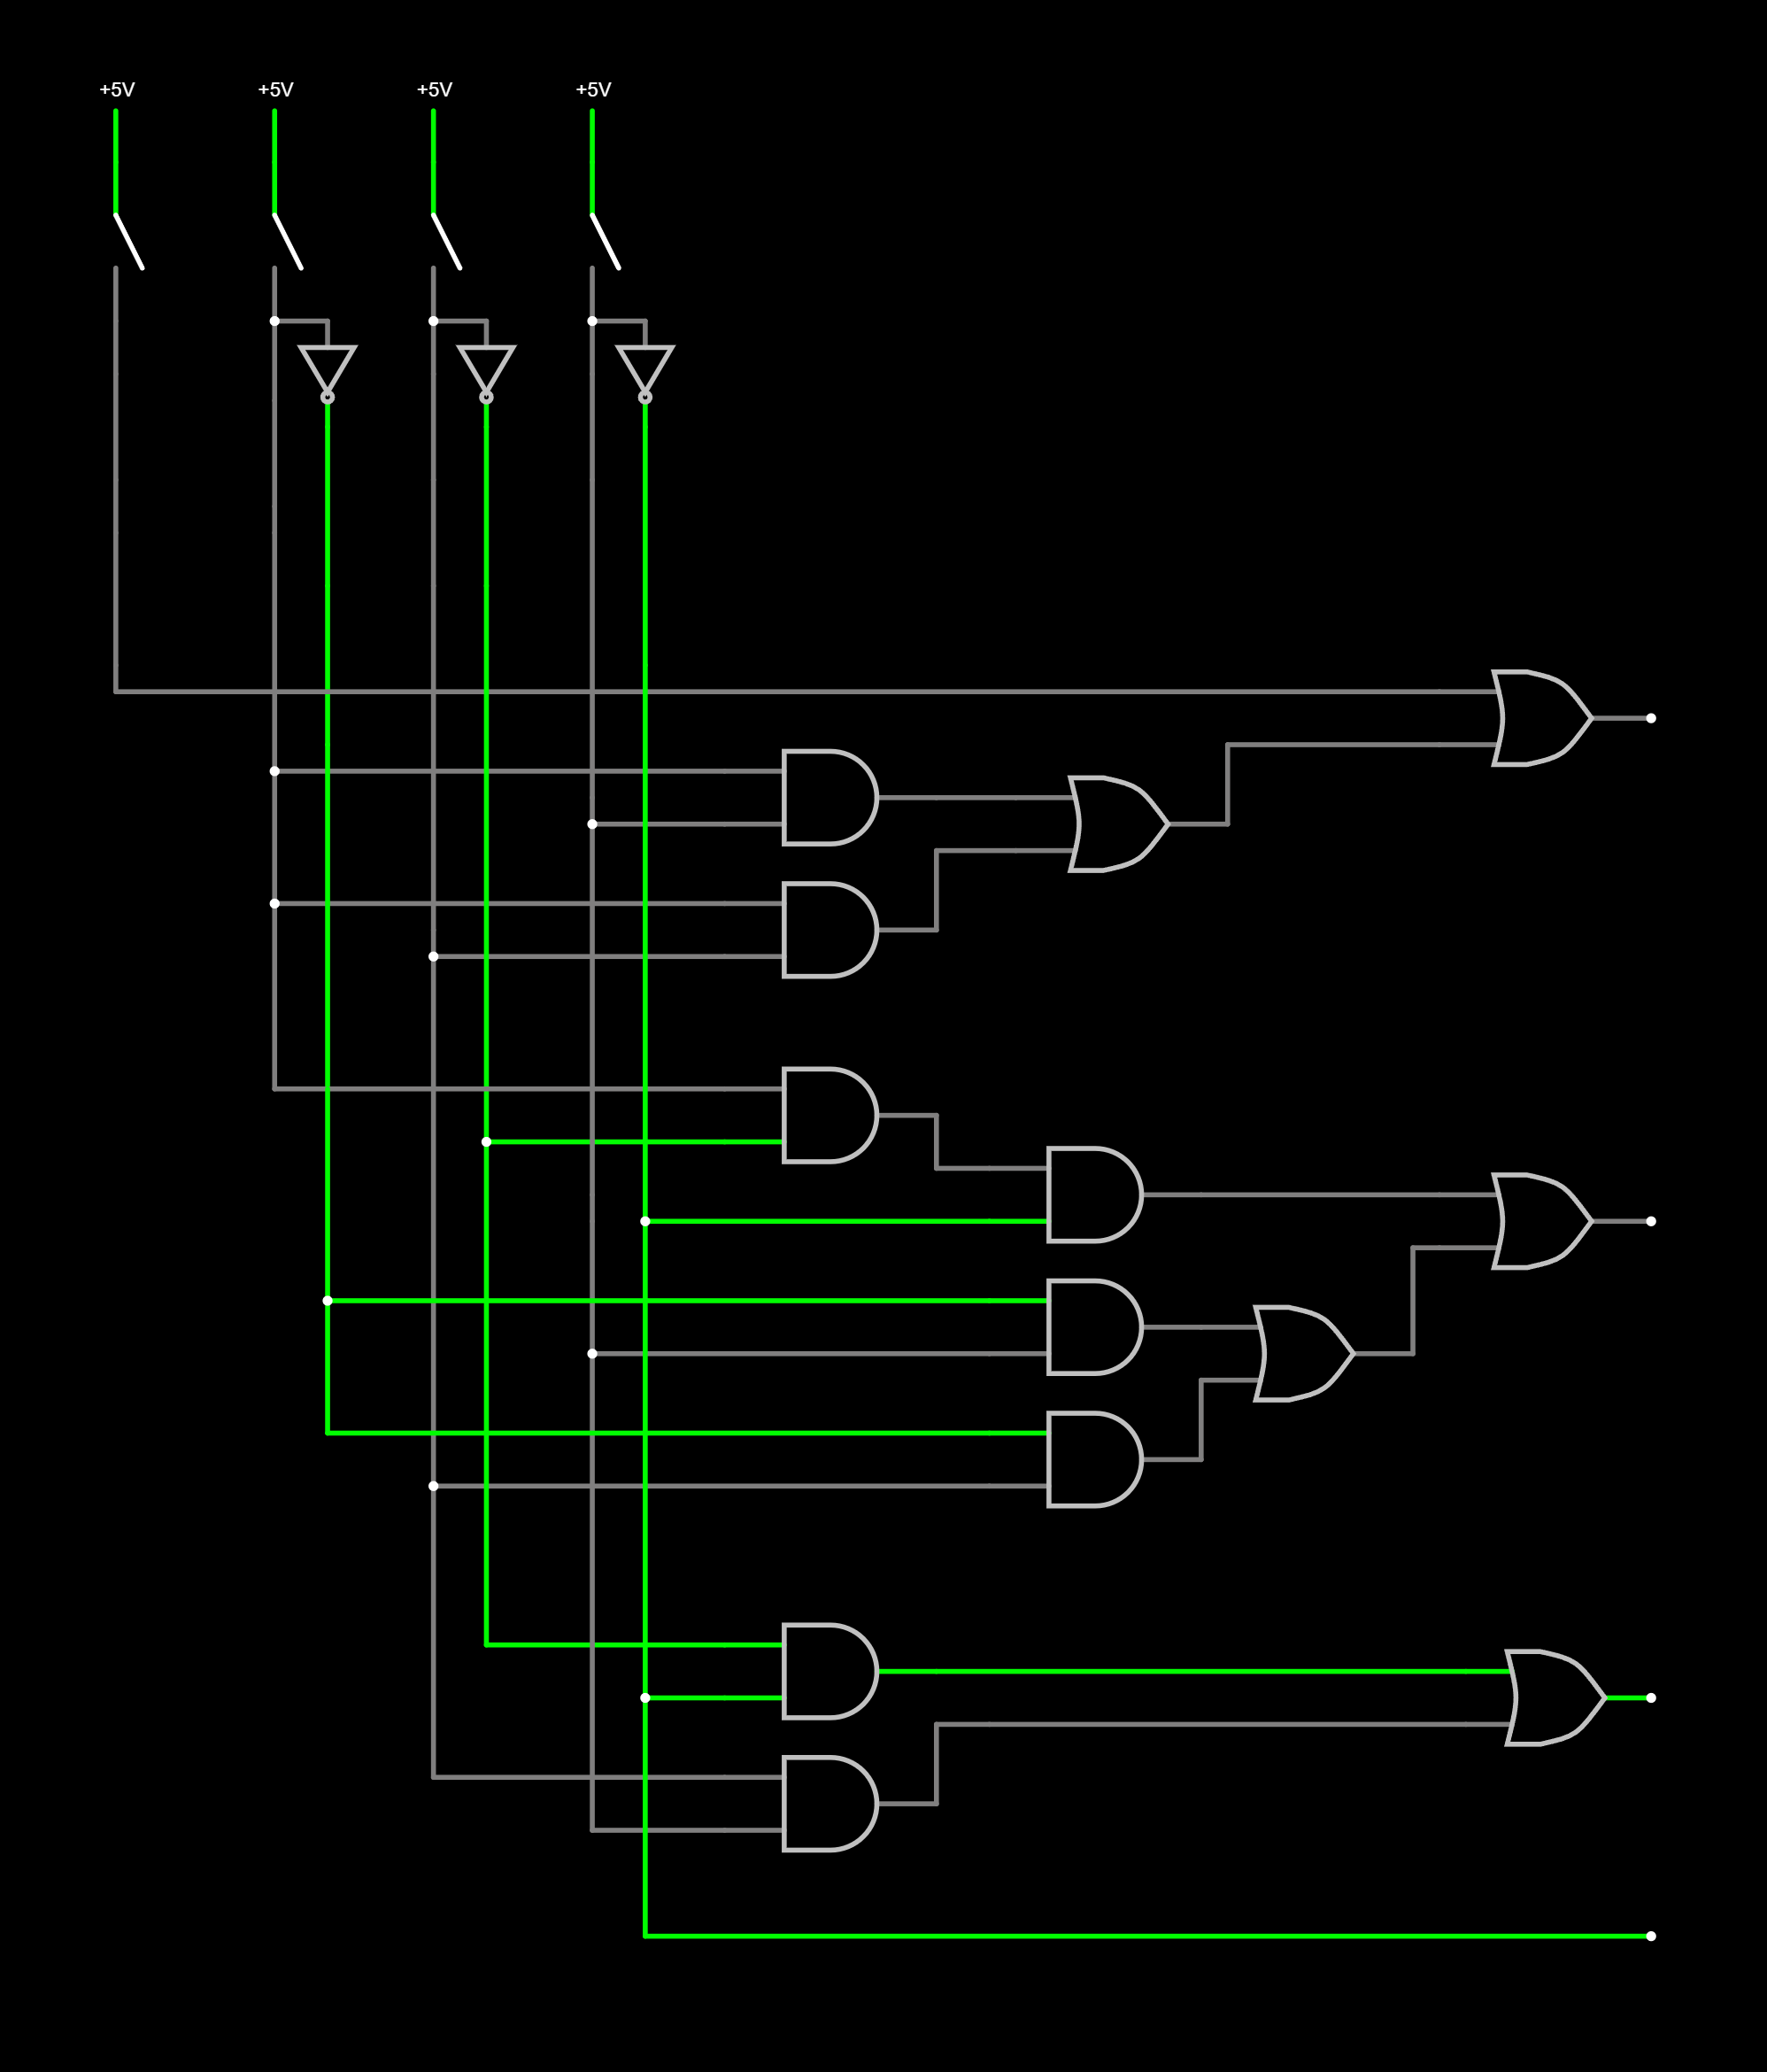
\includegraphics[width=0.5\linewidth]{pictures/simulacion-ej1.png}
        \caption{Imagen de la simulación en la web Falstad.}
        \label{fig:enter-label}
    \end{figure}

    \section{Implementación y verificación con Minilab}
    Luego de verificar el correcto funcionamiento del circuito con un simulador, podemos proceder a implementar el mismo en una placa de pruebas. Luego, con la utilización del Minilab que hemos diseñado y construido, obtendremos las entradas necesarias para el circuito, y podremos visualizar conectados las salidas del mismo nuevamente al Minilab.

    \begin{figure}[H]
        \centering
        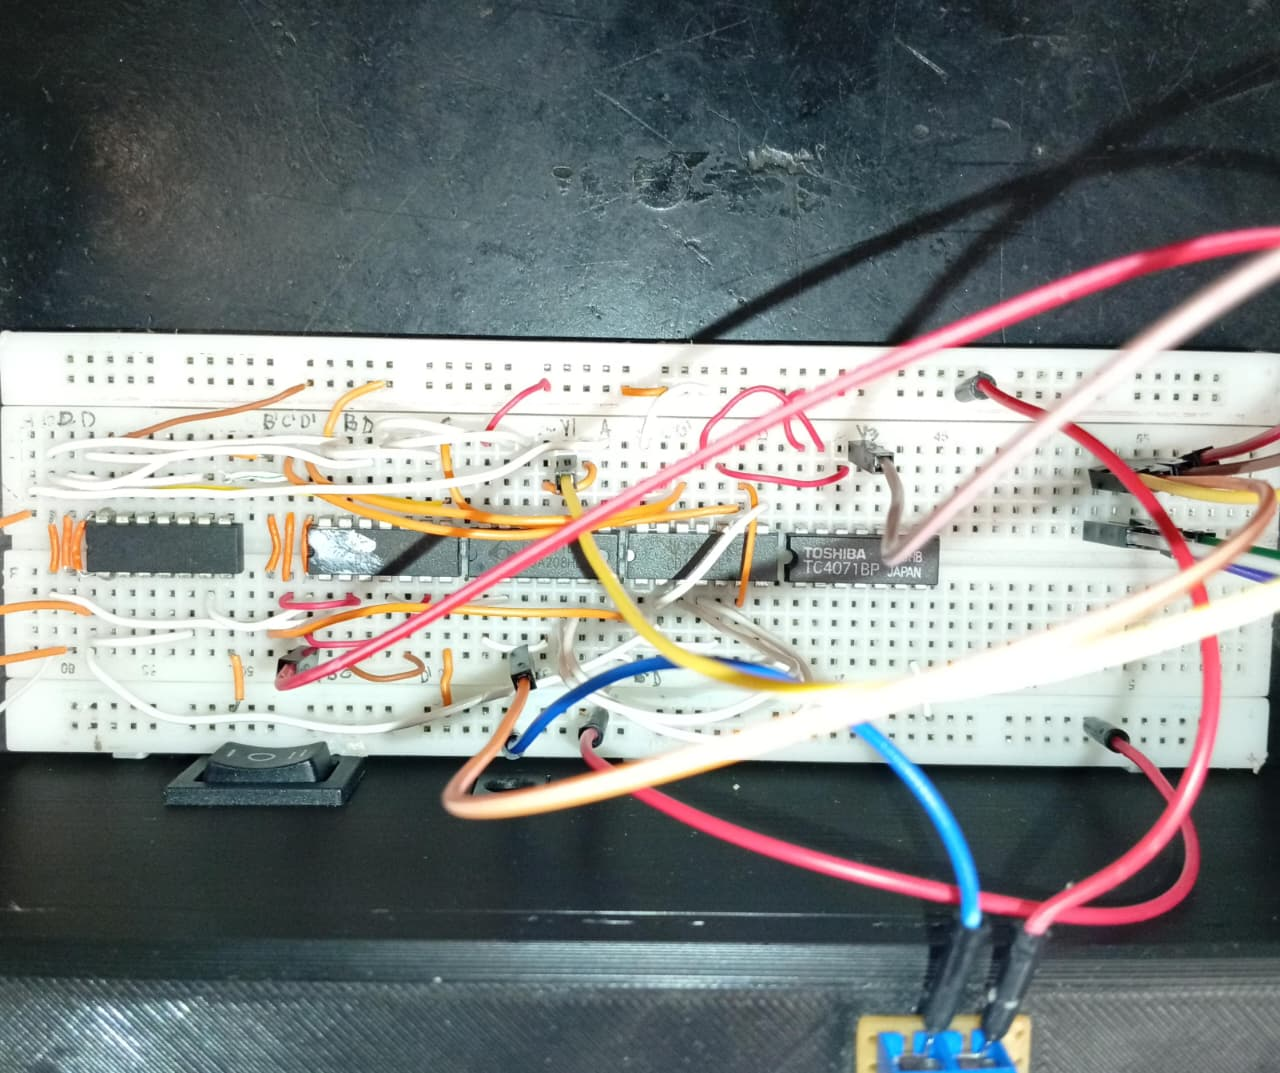
\includegraphics[width=0.8\linewidth]{pictures/circuito1.jpg}
        \caption{Circuito implementado en minlab.}
        \label{fig:enter-label}
    \end{figure}

\chapter{Comparador binario}

El comparador binario consta de tres salidas las cuales van a representar las tres distintas posibilidades de comparacion entre dos numeros de dos bits en las entradas. Las entradas se componenen de A y B, ambos de dos bits. La primer salida $S_0$ va a ser 1 cuando $A>B$, la segunda salida $S_1$ va a ser 1 cuando $A<B$ y por ultimo $S_2$ va a ser 1 cuando ambos numeros sean iguales. 

\section{Tabla de verdad}

\begin{table}[h]
  \centering
  \begin{tabular}{cccc|ccc}
    $A_0$ & $A_1$ & $B_0$ & $B_1$ & $S_0$ & $S_1$ & $S_2$\\
    \hline
    0 & 0 & 0 & 0 & 0 & 0 & 1\\
    0 & 0 & 0 & 1 & 0 & 1 & 0\\
    0 & 0 & 1 & 0 & 0 & 1 & 0\\
    0 & 0 & 1 & 1 & 0 & 1 & 0\\
    0 & 1 & 0 & 0 & 1 & 0 & 0\\
    0 & 1 & 0 & 1 & 0 & 0 & 1\\
    0 & 1 & 1 & 0 & 0 & 1 & 0\\
    0 & 1 & 1 & 1 & 0 & 1 & 0\\
    1 & 0 & 0 & 0 & 1 & 0 & 0\\
    1 & 0 & 0 & 1 & 1 & 0 & 0\\
    1 & 0 & 1 & 0 & 0 & 0 & 1\\
    1 & 0 & 1 & 1 & 0 & 1 & 0\\
    1 & 1 & 0 & 0 & 1 & 0 & 0\\
    1 & 1 & 0 & 1 & 1 & 0 & 0\\
    1 & 1 & 1 & 0 & 1 & 0 & 0\\
    1 & 1 & 1 & 1 & 0 & 0 & 1\\
  \end{tabular}
  \caption{Tabla de verdad del comparador binario}
\end{table}

\section{Obtener las funciones logicas de salidas con circuitos combinacionales}

\begin{equation*}
  S_0=\sum(4,8,9,12,13,14)
\end{equation*}
\begin{equation*}
  S_1=\sum(1,2,3,6,7,11)
\end{equation*}
\begin{equation*}
  S_2=\sum(0,5,10,15)
\end{equation*}

\section{Minimizar utilizando mapas de Karnaugh}
    \begin{tabular}{cc}
      % Primer mapa
      \begin{minipage}{0.45\textwidth}
        \centering
        \begin{karnaugh-map}[4][4][1][$B_1$][$B_0$][$A_1$][$A_0$]
            \minterms{4,8,9,12,13,14}
            \implicant{12}{9}
            \implicant{4}{12}
            \implicantedge{12}{12}{14}{14}
        \end{karnaugh-map}
        \vspace{0.5em}
        $\displaystyle S_0 = A_0 \cdot \overline{B_0} + A_1 \cdot \overline{B_0} \cdot \overline{B_1} + A_0 \cdot A_1 \cdot \overline{B_1}$
      \end{minipage}
      &
      % Segundo mapa
      \begin{minipage}{0.45\textwidth}
        \centering
        \begin{karnaugh-map}[4][4][1][$B_1$][$B_0$][$A_1$][$A_0$]
            \minterms{1,2,3,6,7,11}
            \implicant{1}{3}
            \implicant{3}{6}
            \implicantedge{3}{3}{11}{11}
        \end{karnaugh-map}
        \vspace{0.5em}
        $\displaystyle S_1 = \overline{A_0} \cdot B_0 + \overline{A_0} \cdot \overline{A_1} \cdot B_1 + \overline{A_1} \cdot B_0 \cdot B_1$
      \end{minipage}
      \\[1.5em]
      % Tercer mapa
      \begin{minipage}{0.45\textwidth}
        \centering
        \begin{karnaugh-map}[4][4][1][$B_1$][$B_0$][$A_1$][$A_0$]
            \minterms{0,5,15,10}
            \implicant{0}{0}
            \implicant{5}{5}
            \implicant{15}{15}
            \implicant{10}{10}
        \end{karnaugh-map}
        \vspace{0.5em}
        $\displaystyle S_2 = \overline{A_0} \cdot \overline{A_1} \cdot \overline{B_0} \cdot \overline{B_1} + \overline{A_0} \cdot A_1 \cdot \overline{B_0} \cdot B_1 + A_0 \cdot A_1 \cdot B_0 \cdot B_1 + A_0 \cdot \overline{A_1} \cdot B_0 \cdot \overline{B_1}$
      \end{minipage}
    \end{tabular}

\section{Implementación con compuertas}

    \begin{figure}[H]
      \centering
      \tikzset{
      logic gate style/.style={scale=1.5, transform shape}
      }
      \begin{circuitikz}[circuit logic US]
        \node at (0,0) [](A){$A_0$};
        \node at (1,0) [](B){$A_1$};
        \node at (2,0) [](C){$B_0$};
        \node at (3,0) [](D){$B_1$};

        \node[not gate, draw, scale=0.5, transform shape, rotate=-90] (NotA) at ($(A)+(0.5,-0.8)$) {};
        \draw (A)  to[short] ++ (0,-17.5) coordinate (end);
        \draw ($(A)+(0,-0.5)$)  -| (NotA.input);
        \draw (NotA.output)  to[short] ($(NotA.output |- end)$);

        \node[not gate, draw, scale=0.5, transform shape, rotate=-90] (NotB) at ($(B)+(0.5,-0.8)$) {};
        \draw (B)  to[short] ($(B |- end)$);
        \draw ($(B)+(0,-0.5)$)  -| (NotB.input);
        \draw (NotB.output)  to[short] ($(NotB.output |- end)$);

        \node[not gate, draw, scale=0.5, transform shape, rotate=-90] (NotC) at ($(C)+(0.5,-0.8)$) {};
        \draw (C)  to[short] ($(C |- end)$);
        \draw ($(C)+(0,-0.5)$)  -| (NotC.input);
        \draw (NotC.output)  to[short] ($(NotC.output |- end)$);

        \node[not gate, draw, scale=0.5, transform shape, rotate=-90] (NotD) at ($(D)+(0.5,-0.8)$) {};
        \draw (D)  to[short] ($(D |- end)$);
        \draw ($(D)+(0,-0.5)$)  -| (NotD.input);
        \draw (NotD.output)  to[short] ($(NotD.output |- end)$);

        % S1 ---------------------------------------------------------
        \node[and gate] (A1) at (5,-2) {};
        \node[and gate] (A2) at (5,-3) {};
        \node[and gate] (A3) at (5,-4.5) {};
        \node[and gate] (A4) at (6.5,-3.75) {};
        \node[and gate] (A5) at (6.5,-5) {};
        \node[or gate] (O1) at (8,-2.5) {};
        \node[or gate] (O2) at (9.5,-3.5) {};

        \draw ($(A |- A1.input 1)$)  to[short, *-] (A1.input 1);
        \draw ($(NotC |- A1.input 2)$)  to[short, *-] (A1.input 2);
        \draw ($(B |- A2.input 1)$)  to[short, *-] (A2.input 1);
        \draw ($(NotC |- A2.input 2)$)  to[short, *-] (A2.input 2);
        \draw ($(A |- A3.input 1)$)  to[short, *-] (A3.input 1);
        \draw ($(B |- A3.input 2)$)  to[short, *-] (A3.input 2);
        \draw (A2.output) -- ++(0.3,0) |- (A4.input 1);
        \draw ($(NotD |- A4.input 2)$)  to[short, *-] (A4.input 2);
        \draw (A3.output) -- ++(0.3,0) |- (A5.input 1);
        \draw ($(NotD |- A5.input 2)$)  to[short, *-] (A5.input 2);
        \draw (A1.output) -- ++(0.3,0) |- (O1.input 1);
        \draw (A4.output) -- ++(0.3,0) |- (O1.input 2);
        \draw (O1.output) -- ++(0.3,0) |- (O2.input 1);
        \draw (A5.output) -- ++(1,0) |- (O2.input 2);

        \node at ($(O2.output) + (3,0)$) [](S1){$S_1$};
        \draw (O2.output) -- (S1) coordinate (salidas);

        % S2 ---------------------------------------------------------
        \node[and gate] (A1) at (5,-6) {};
        \node[and gate] (A2) at (5,-7) {};
        \node[and gate] (A3) at (5,-8.5) {};
        \node[and gate] (A4) at (6.5,-7.75) {};
        \node[and gate] (A5) at (6.5,-9) {};
        \node[or gate] (O1) at (8,-6.5) {};
        \node[or gate] (O2) at (9.5,-7.5) {};

        \draw ($(NotA |- A1.input 1)$)  to[short, *-] (A1.input 1);
        \draw ($(C |- A1.input 2)$)  to[short, *-] (A1.input 2);
        \draw ($(NotA |- A2.input 1)$)  to[short, *-] (A2.input 1);
        \draw ($(NotB |- A2.input 2)$)  to[short, *-] (A2.input 2);
        \draw ($(NotB |- A3.input 1)$)  to[short, *-] (A3.input 1);
        \draw ($(C |- A3.input 2)$)  to[short, *-] (A3.input 2);
        \draw (A2.output) -- ++(0.3,0) |- (A4.input 1);
        \draw ($(D |- A4.input 2)$)  to[short, *-] (A4.input 2);
        \draw (A3.output) -- ++(0.3,0) |- (A5.input 1);
        \draw ($(D |- A5.input 2)$)  to[short, *-] (A5.input 2);
        \draw (A1.output) -- ++(0.3,0) |- (O1.input 1);
        \draw (A4.output) -- ++(0.3,0) |- (O1.input 2);
        \draw (O1.output) -- ++(0.3,0) |- (O2.input 1);
        \draw (A5.output) -- ++(1,0) |- (O2.input 2);

        \node at ($(O2.output) + (3,0)$) [](S2){$S_2$};
        \draw (O2.output) -- (S2) coordinate (salidas);

        % S3 ---------------------------------------------------------
        \node[and gate] (A1) at (5,-10) {};
        \node[and gate] (A2) at (6.5,-10.5) {};
        \node[and gate] (A3) at (8,-11) {};
        \node[and gate] (A4) at (5,-12) {};
        \node[and gate] (A5) at (6.5,-12.5) {};
        \node[and gate] (A6) at (8,-13) {};
        \node[and gate] (A7) at (5,-14) {};
        \node[and gate] (A8) at (6.5,-14.5) {};
        \node[and gate] (A9) at (8,-15) {};
        \node[and gate] (A10) at (5,-16) {};
        \node[and gate] (A11) at (6.5,-16.5) {};
        \node[and gate] (A12) at (8,-17) {};
        \node[or gate] (O1) at (9.5,-12) {};
        \node[or gate] (O2) at (9.5,-16) {};
        \node[or gate] (O3) at (11,-14) {};

        \draw ($(NotD |- A1.input 1)$)  to[short, *-] (A1.input 1);
        \draw ($(NotC |- A1.input 2)$)  to[short, *-] (A1.input 2);
        \draw (A1.output) -- ++(0.3,0) |- (A2.input 1);
        \draw ($(NotB |- A2.input 2)$)  to[short, *-] (A2.input 2);
        \draw (A2.output) -- ++(0.3,0) |- (A3.input 1);
        \draw ($(NotA |- A3.input 2)$)  to[short, *-] (A3.input 2);

        \draw ($(D |- A4.input 1)$)  to[short, *-] (A4.input 1);
        \draw ($(NotC |- A4.input 2)$)  to[short, *-] (A4.input 2);
        \draw (A4.output) -- ++(0.3,0) |- (A5.input 1);
        \draw ($(B |- A5.input 2)$)  to[short, *-] (A5.input 2);
        \draw (A5.output) -- ++(0.3,0) |- (A6.input 1);
        \draw ($(NotA |- A6.input 2)$)  to[short, *-] (A6.input 2);

        \draw ($(D |- A7.input 1)$)  to[short, *-] (A7.input 1);
        \draw ($(C |- A7.input 2)$)  to[short, *-] (A7.input 2);
        \draw (A7.output) -- ++(0.3,0) |- (A8.input 1);
        \draw ($(B |- A8.input 2)$)  to[short, *-] (A8.input 2);
        \draw (A8.output) -- ++(0.3,0) |- (A9.input 1);
        \draw ($(A |- A9.input 2)$)  to[short, *-] (A9.input 2);

        \draw ($(NotD |- A10.input 1)$)  to[short, *-] (A10.input 1);
        \draw ($(C |- A10.input 2)$)  to[short, *-] (A10.input 2);
        \draw (A10.output) -- ++(0.3,0) |- (A11.input 1);
        \draw ($(NotB |- A11.input 2)$)  to[short, *-] (A11.input 2);
        \draw (A11.output) -- ++(0.3,0) |- (A12.input 1);
        \draw ($(A |- A12.input 2)$)  to[short, *-] (A12.input 2);

        \draw (A3.output) -- ++(0.3,0) |- (O1.input 1);
        \draw (A6.output) -- ++(0.3,0) |- (O1.input 2);
        \draw (A9.output) -- ++(0.3,0) |- (O2.input 1);
        \draw (A12.output) -- ++(0.3,0) |- (O2.input 2);
        \draw (O1.output) -- ++(0.3,0) |- (O3.input 1);
        \draw (O2.output) -- ++(0.3,0) |- (O3.input 2);

        \node at ($(O3.output) + (1.5,0)$) [](S3){$S_3$};
        \draw (O3.output) -- (S3) coordinate (salidas);

      \end{circuitikz}
      \caption{Implementación con compuertas}
    \end{figure}

\section{Armado de circuito y verificacion en el minilab}

Una vez armado el circuito como indica en la imagen procedemos a verificarlo en el minilab.

  \begin{figure}[H]
      \centering
      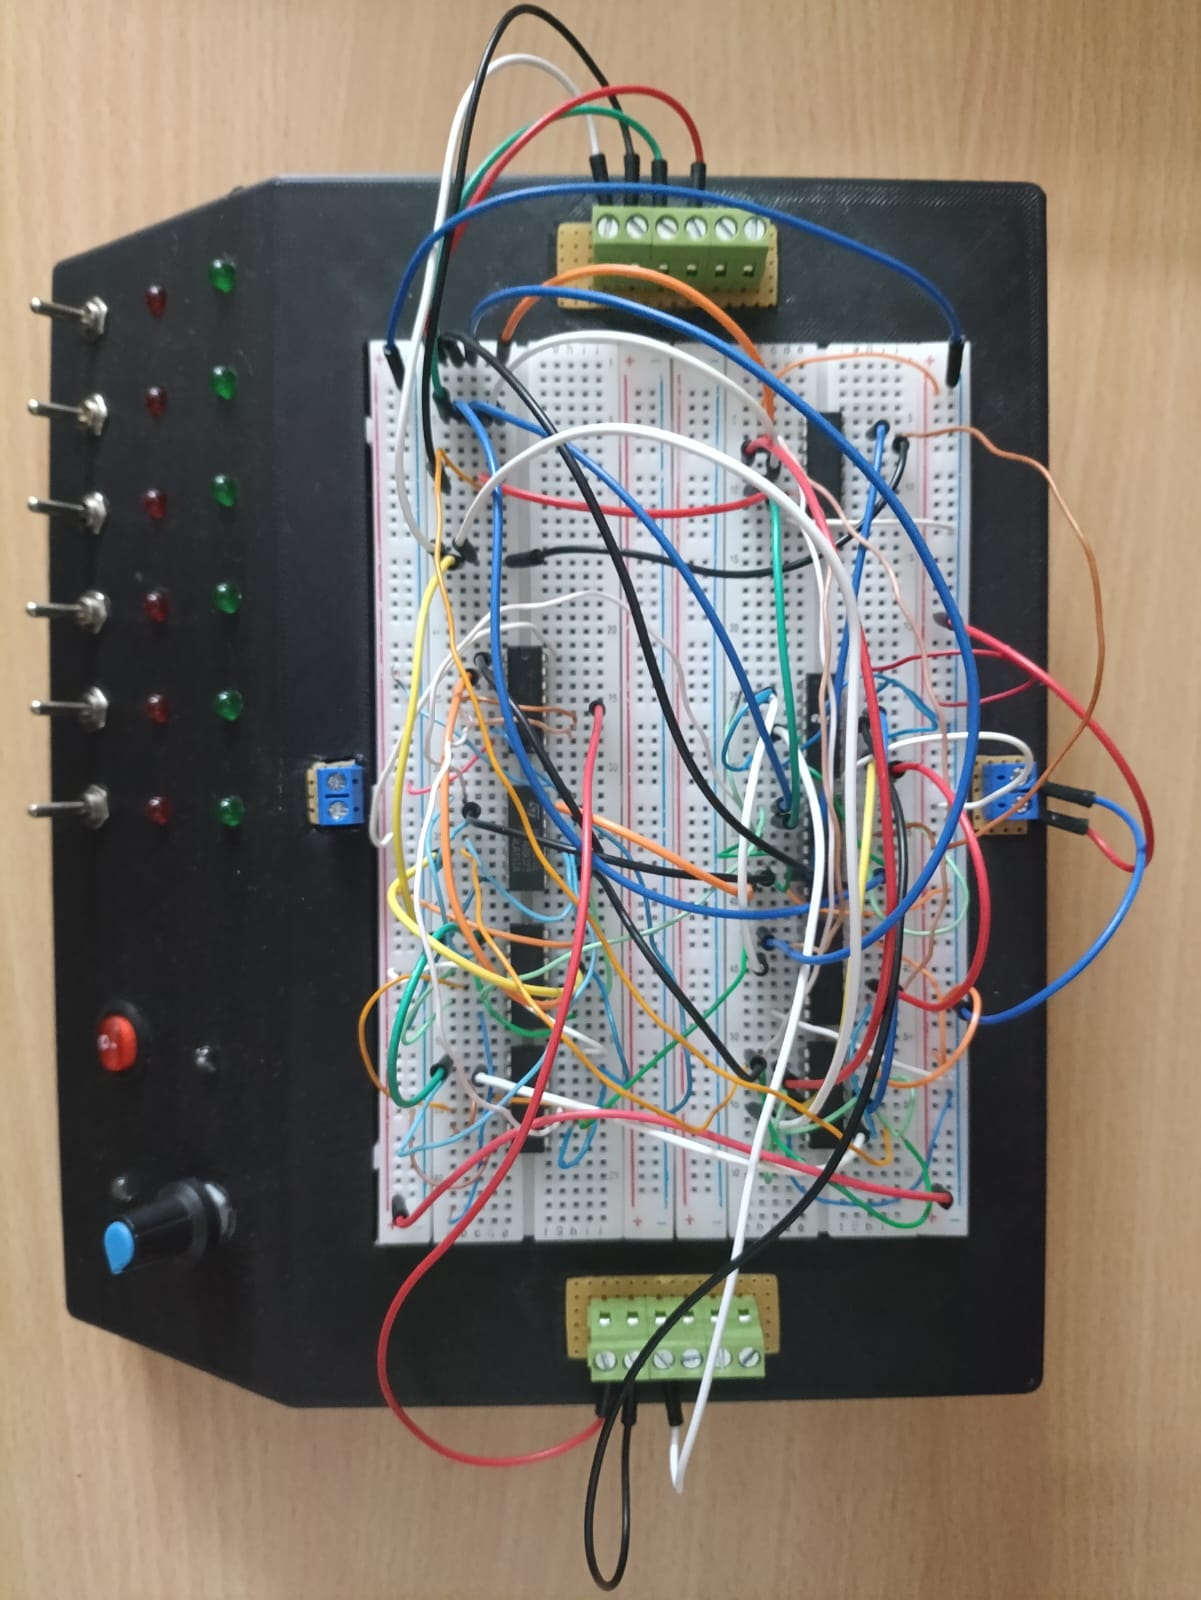
\includegraphics[width=0.8\linewidth]{pictures/circuito2.jpeg}
      \caption{Circuito implementado en minlab.}
      \label{fig:enter-label}
  \end{figure}

\section{Simulacion en falstad}

Por ultimo se utiliza la herramienta falstad de la misma forma hecha anteriormente en el ejercicio 1.

\begin{figure}[h]
  \centering
  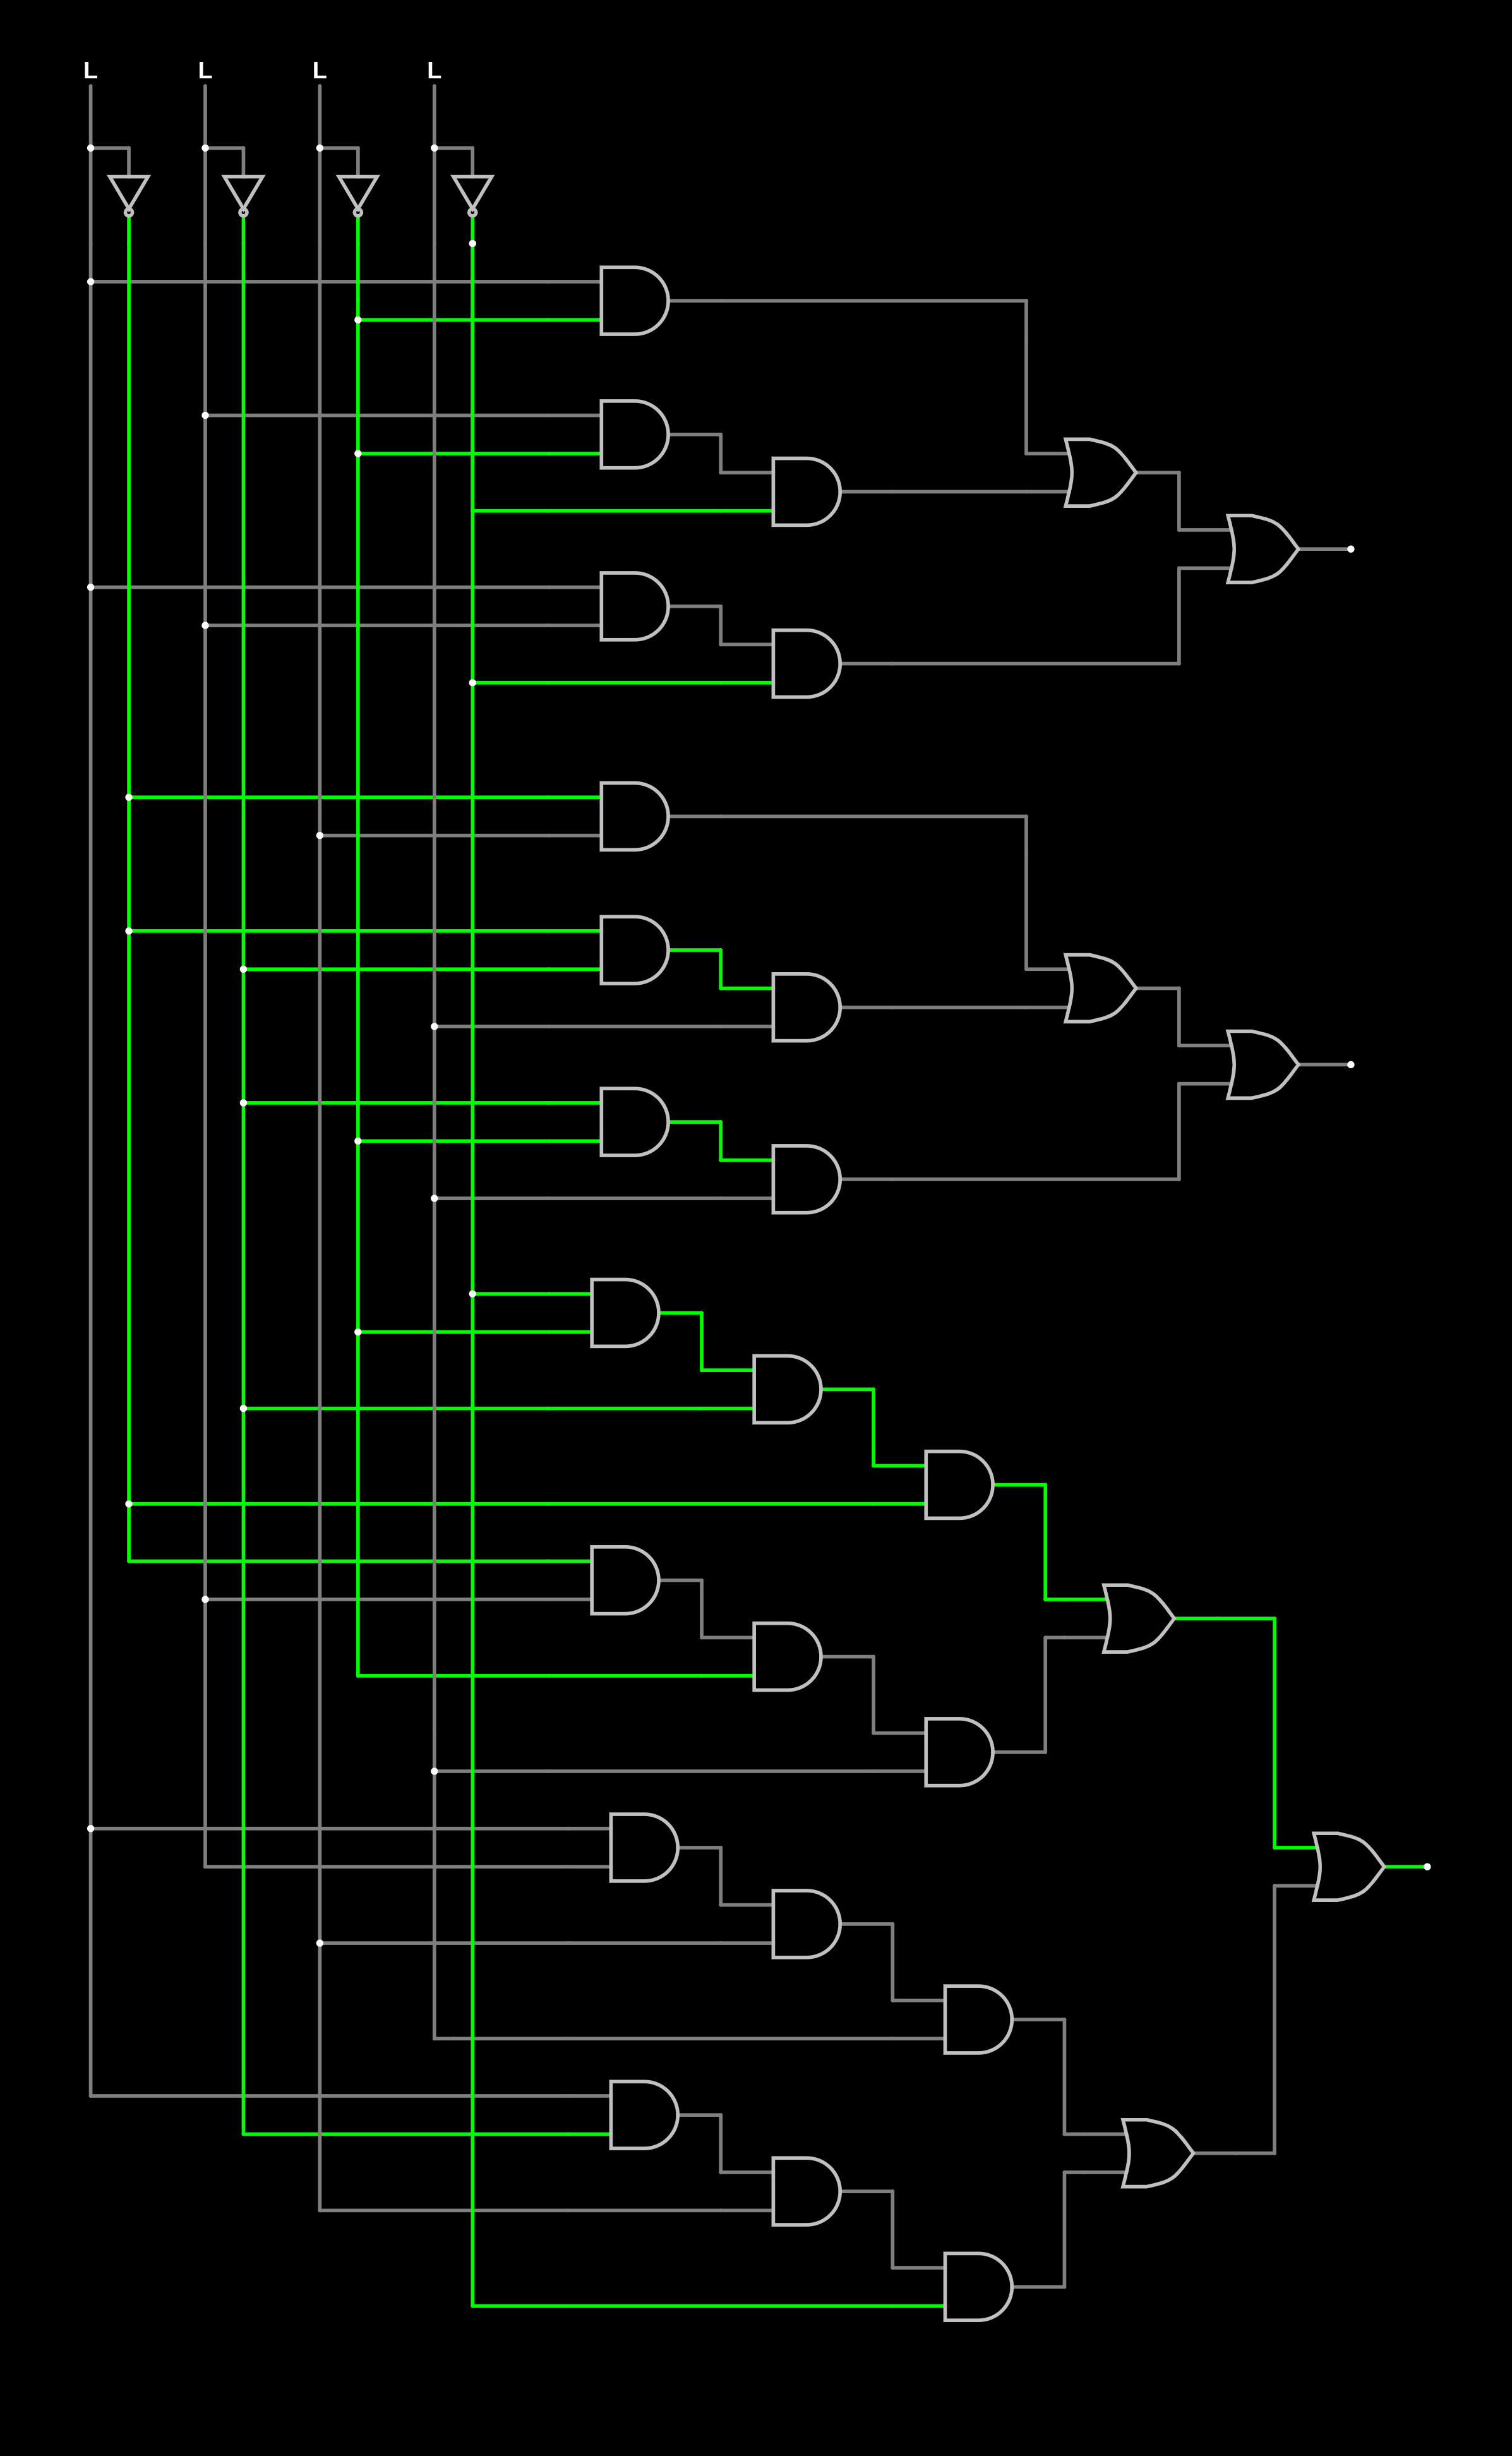
\includegraphics[width=0.5\linewidth]{pictures/simulacion-ej2.png}
  \caption{Imagen de la simulación en la web Falstad.}
  \label{fig:enter-label}
\end{figure}

\chapter{Conclusión}

En este trabajo práctico tuvimos la oportunidad de aplicar en profundidad los conceptos aprendidos sobre mapas de Karnaugh y circuitos combinacionales. A través del diseño de un conversor de BCD a Exceso-3 y un comparador binario, pudimos poner en práctica la simplificación de funciones lógicas, utilizando herramientas como el álgebra de Boole y los mapas de Karnaugh para optimizar las expresiones resultantes.

Este proceso nos permitió reforzar el conocimiento teórico adquirido en clase, llevándolo a un plano más práctico. También nos familiarizamos con la implementación física de los circuitos diseñados, empleando simuladores digitales que facilitaron la verificación del correcto funcionamiento antes de pasar al montaje real.

Uno de los aspectos más desafiantes de este trabajo fue el armado de los circuitos en la protoboard. La cantidad considerable de compuertas lógicas necesarias, junto con la complejidad de las interconexiones entre los distintos circuitos integrados, exige un trabajo meticuloso y organizado. Cualquier error de conexión puede provocar fallas difíciles de detectar si no se sigue un esquema claro y ordenado.

\end{document}
